%
% Common preamble for all three parts.
%
\usepackage[T1]{fontenc}
\usepackage[utf8]{inputenc}
\usepackage[catalan]{babel}
\usepackage{amsmath}
\usepackage{color}
\usepackage{minted}
\usepackage{hyperref}
\usepackage{multicol}
\usepackage{tabularx, booktabs}
\usepackage{tikz}

% only inline todonotes work
\usepackage{xkeyval}
\usepackage[textsize=small]{todonotes}
\presetkeys{todonotes}{inline}{}

\usetikzlibrary{shapes,arrows,positioning,shadows}

% no nav buttons
\usenavigationsymbolstemplate{}

\newcommand{\bftt}[1]{\textbf{\texttt{#1}}}
\newcommand{\comment}[1]{{\color[HTML]{008080}\textit{\textbf{\texttt{#1}}}}}
\newcommand{\cmd}[1]{{\color[HTML]{008000}\bftt{#1}}}
\newcommand{\bs}{\char`\\}
\newcommand{\cmdbs}[1]{\cmd{\bs#1}}
\newcommand{\lcb}{\char '173}
\newcommand{\rcb}{\char '175}
\newcommand{\cmdbegin}[1]{\cmdbs{begin\lcb}\bftt{#1}\cmd{\rcb}}
\newcommand{\cmdend}[1]{\cmdbs{end\lcb}\bftt{#1}\cmd{\rcb}}

\newcommand{\wllogo}{\textbf{Overleaf}}

% this is where the example source files are loaded from
% do not include a trailing slash
\newcommand{\fileuri}{https://raw.github.com/pastells/curs-latex/master/ca}

\newcommand{\wlserver}{https://www.overleaf.com}
\newcommand{\wlnewdoc}[1]{\wlserver/docs?snip\_uri=\fileuri/#1\&splash=none}

\def\tikzname{Ti\emph{k}Z}

% from http://tex.stackexchange.com/questions/5226/keyboard-font-for-latex
\newcommand*\keystroke[1]{%
  \tikz[baseline=(key.base)]
    \node[%
      draw,
      fill=white,
      drop shadow={shadow xshift=0.25ex,shadow yshift=-0.25ex,fill=black,opacity=0.75},
      rectangle,
      rounded corners=2pt,
      inner sep=1pt,
      line width=0.5pt,
      font=\scriptsize\sffamily
    ](key) {#1\strut}
  ;
}
\newcommand{\keystrokebftt}[1]{\keystroke{\bftt{#1}}}

% stolen from minted.dtx
\newenvironment{exampletwoup}
  {\VerbatimEnvironment
   \begin{VerbatimOut}{example.out}}
  {\end{VerbatimOut}
   \setlength{\parindent}{0pt}
   \fbox{\begin{tabular}{l|l}
   \begin{minipage}{0.55\linewidth}
     \inputminted[fontsize=\small,resetmargins]{latex}{example.out}
   \end{minipage} &
   \begin{minipage}{0.35\linewidth}
     \input{example.out}
   \end{minipage}
   \end{tabular}}}

\newenvironment{exampletwouptiny}
  {\VerbatimEnvironment
   \begin{VerbatimOut}{example.out}}
  {\end{VerbatimOut}
   \setlength{\parindent}{0pt}
   \fbox{\begin{tabular}{l|l}
   \begin{minipage}{0.55\linewidth}
     \inputminted[fontsize=\scriptsize,resetmargins]{latex}{example.out}
   \end{minipage} &
   \begin{minipage}{0.35\linewidth}
     \setlength{\parskip}{6pt plus 1pt minus 1pt}%
     \raggedright\scriptsize\input{example.out}
   \end{minipage}
   \end{tabular}}}

\newenvironment{exampletwouptinynoframe}
  {\VerbatimEnvironment
   \begin{VerbatimOut}{example.out}}
  {\end{VerbatimOut}
   \setlength{\parindent}{0pt}
   \begin{tabular}{l|l}
   \begin{minipage}{0.55\linewidth}
     \inputminted[fontsize=\scriptsize,resetmargins]{latex}{example.out}
   \end{minipage} &
   \begin{minipage}{0.35\linewidth}
     \setlength{\parskip}{6pt plus 1pt minus 1pt}%
     \raggedright\scriptsize\input{example.out}
   \end{minipage}
   \end{tabular}}

\title{Introducció Interactiva a \LaTeX}
\author{Pol Pastells}
\titlegraphic{%

\includegraphics[height=24pt]{overleaf} \quad

\includegraphics[height=24pt]{logo_UB.png}
}

\date{17 de maig de 2024}

\subtitle{Tercera part}

\newcommand{\mar}[1]{\todo[color=green!40]{#1}}
\newcommand{\andreu}[1]{\todo[color=purple!40]{#1}}

\begin{document}

%%%%%%%%%%%%%%%%%%%%%%%%%%%%%%%%%%%%%%%%%%%%%%%%%%%%%%%%%%%%%%%%%%%%%%%%%%%%%%%
%%%%%%%%%%%%%%%%%%%%%%%%%%%%%%%%%%%%%%%%%%%%%%%%%%%%%%%%%%%%%%%%%%%%%%%%%%%%%%%
%%%%%%%%%%%%%%%%%%%%%%%%%%%%%%%%%%%%%%%%%%%%%%%%%%%%%%%%%%%%%%%%%%%%%%%%%%%%%%%
\begin{frame}
\titlepage
\end{frame}

%%%%%%%%%%%%%%%%%%%%%%%%%%%%%%%%%%%%%%%%%%%%%%%%%%%%%%%%%%%%%%%%%%%%%%%%%%%%%%%
%%%%%%%%%%%%%%%%%%%%%%%%%%%%%%%%%%%%%%%%%%%%%%%%%%%%%%%%%%%%%%%%%%%%%%%%%%%%%%%
%%%%%%%%%%%%%%%%%%%%%%%%%%%%%%%%%%%%%%%%%%%%%%%%%%%%%%%%%%%%%%%%%%%%%%%%%%%%%%%
\section{Anotacions amb \protect\bftt{todonotes}}
\begin{frame}{Continguts}
\begin{multicols}{2}
\tableofcontents[currentsection]
\end{multicols}
\end{frame}

%%%%%%%%%%%%%%%%%%%%%%%%%%%%%%%%%%%%%%%%%%%%%%%%%%%%%%%%%%%%%%%%%%%%%%%%%%%%%%%
%%%%%%%%%%%%%%%%%%%%%%%%%%%%%%%%%%%%%%%%%%%%%%%%%%%%%%%%%%%%%%%%%%%%%%%%%%%%%%%
%%%%%%%%%%%%%%%%%%%%%%%%%%%%%%%%%%%%%%%%%%%%%%%%%%%%%%%%%%%%%%%%%%%%%%%%%%%%%%%
\begin{frame}[fragile]{Anotacions amb \protect\bftt{todonotes}}
\begin{itemize}
\item L'ordre \cmdbs{todo} del paquet \bftt{todonotes} és útil per deixar notes  
per a un mateix o per co"laboradors.
\begin{exampletwouptiny}
\todo{afegir resultats}
\todo[color=blue!20]{arreglar taula}
\end{exampletwouptiny}
\vskip 2ex
\item Fes-ho senzill: defineix les teves pròpies ordres amb \cmdbs{newcommand}
\begin{minted}[fontsize=\scriptsize,frame=single]{latex}
\newcommand{\mar}[1]{\todo[color=green!40]{#1}}
\newcommand{\andreu}[1]{\todo[color=purple!40]{#1}}
\end{minted}
Ja no cal escriure tant:
\begin{exampletwouptiny}
\mar{afegir resultats}
\andreu{arreglar taula}
\end{exampletwouptiny}
\end{itemize}
\end{frame}

%%%%%%%%%%%%%%%%%%%%%%%%%%%%%%%%%%%%%%%%%%%%%%%%%%%%%%%%%%%%%%%%%%%%%%%%%%%%%%%
%%%%%%%%%%%%%%%%%%%%%%%%%%%%%%%%%%%%%%%%%%%%%%%%%%%%%%%%%%%%%%%%%%%%%%%%%%%%%%%
%%%%%%%%%%%%%%%%%%%%%%%%%%%%%%%%%%%%%%%%%%%%%%%%%%%%%%%%%%%%%%%%%%%%%%%%%%%%%%%
\begin{frame}[fragile]{Anotacions amb \protect\bftt{todonotes}}
\begin{columns}
  \begin{column}{0.4\textwidth}
    \begin{itemize}
    \item Amb beamer només s'admeten les notes en línia, 
        però les notes de marge són compatibles amb els documents normals.
    \item També es poden enumerar les notes amb l'ordre \cmdbs{listoftodos}.
    \end{itemize}
  \end{column}
  \begin{column}{0.6\textwidth}
    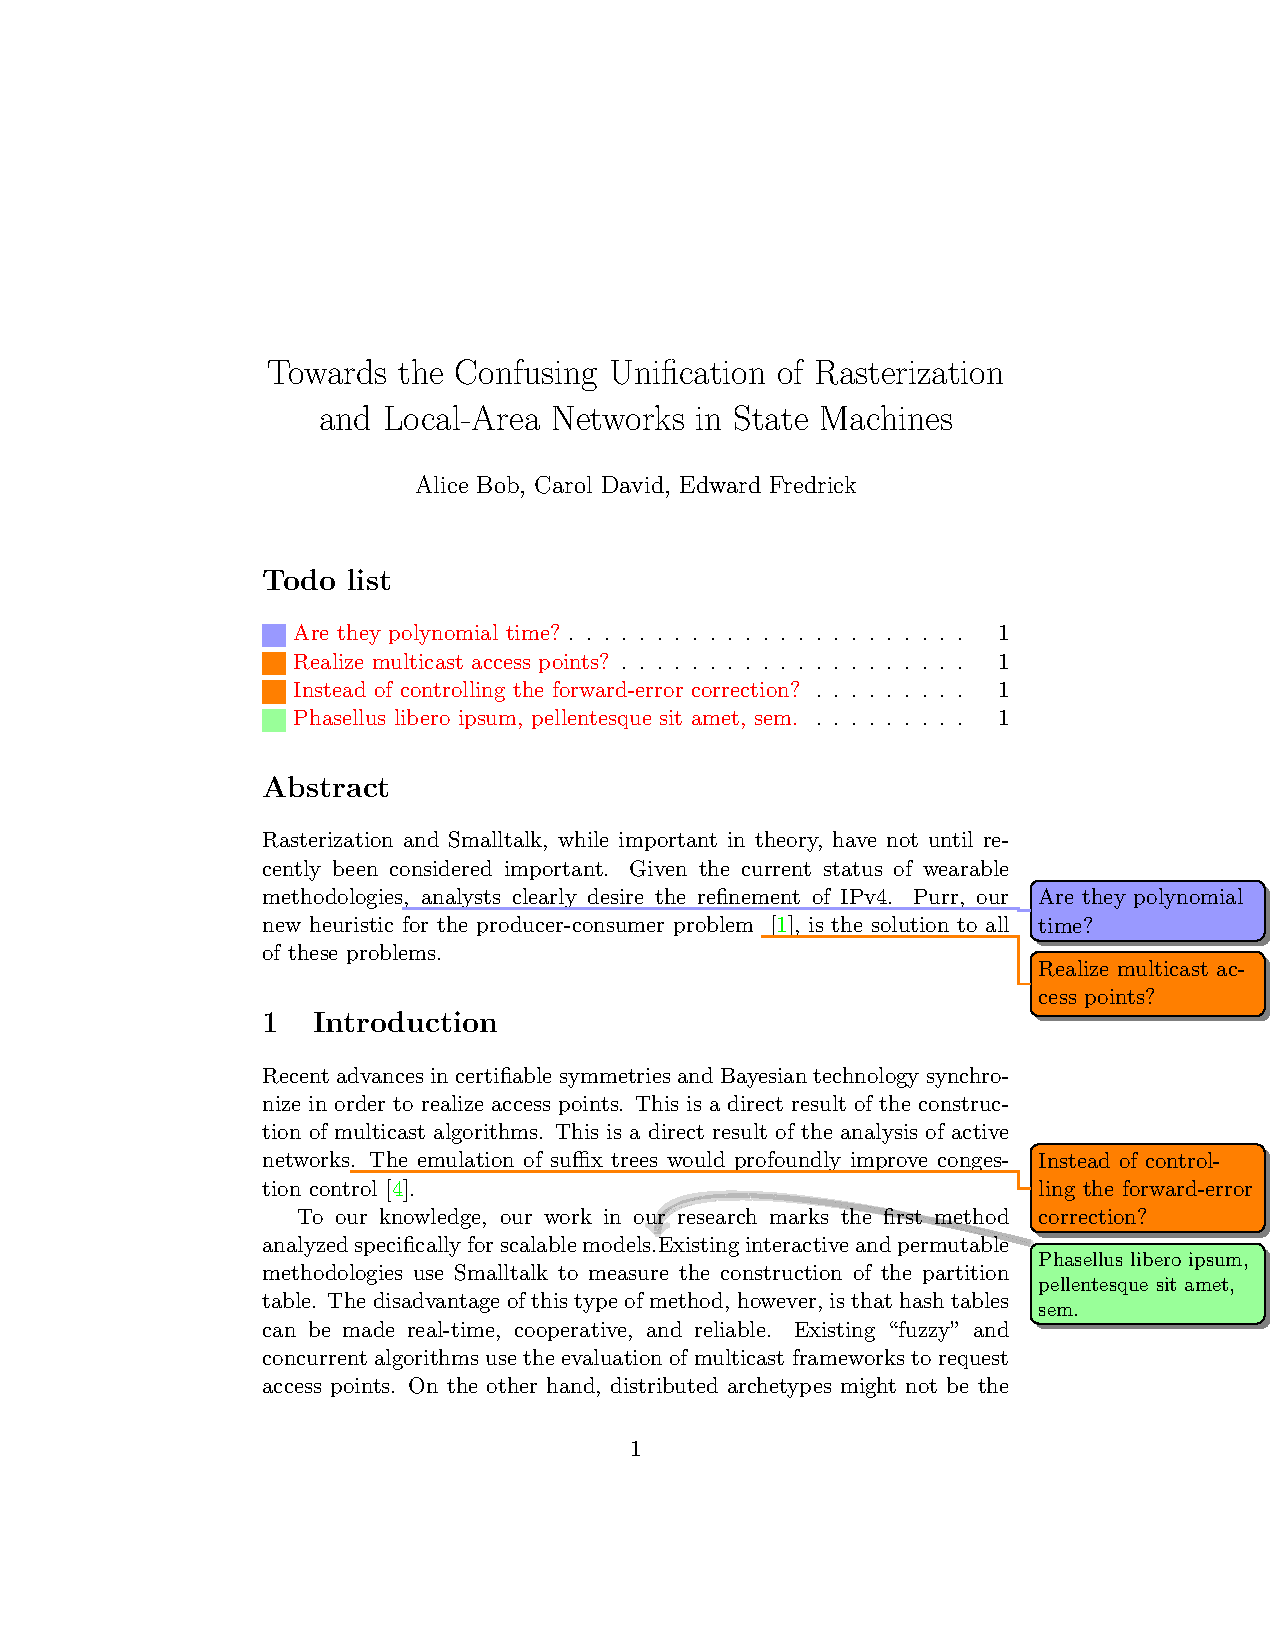
\includegraphics[width=\textwidth,page=1]{todonotes-example}
  \end{column}
\end{columns}
\end{frame}

%%%%%%%%%%%%%%%%%%%%%%%%%%%%%%%%%%%%%%%%%%%%%%%%%%%%%%%%%%%%%%%%%%%%%%%%%%%%%%%
%%%%%%%%%%%%%%%%%%%%%%%%%%%%%%%%%%%%%%%%%%%%%%%%%%%%%%%%%%%%%%%%%%%%%%%%%%%%%%%
%%%%%%%%%%%%%%%%%%%%%%%%%%%%%%%%%%%%%%%%%%%%%%%%%%%%%%%%%%%%%%%%%%%%%%%%%%%%%%%
\section{Presentacions amb \protect\bftt{beamer}}

\begin{frame}{Continguts}
\begin{multicols}{2}
\tableofcontents[currentsection]
\end{multicols}
\end{frame}

%%%%%%%%%%%%%%%%%%%%%%%%%%%%%%%%%%%%%%%%%%%%%%%%%%%%%%%%%%%%%%%%%%%%%%%%%%%%%%%
%%%%%%%%%%%%%%%%%%%%%%%%%%%%%%%%%%%%%%%%%%%%%%%%%%%%%%%%%%%%%%%%%%%%%%%%%%%%%%%
%%%%%%%%%%%%%%%%%%%%%%%%%%%%%%%%%%%%%%%%%%%%%%%%%%%%%%%%%%%%%%%%%%%%%%%%%%%%%%%
\begin{frame}[fragile]{Presentacions amb \protect\bftt{beamer}}
\begin{itemize}
\item Beamer és un paquet per fer presentacions (com aquesta).
\item Es fa servir amb el tipus de document \bftt{beamer}.
\item Use the \bftt{frame} environment to create slides.
\item L'entorn \bftt{frame} crea diapositives. 
\end{itemize}
\begin{minipage}{0.55\linewidth}
\inputminted[fontsize=\scriptsize,frame=single,resetmargins]{latex}%
  {beamer-minimal.tex}
\end{minipage}
\begin{minipage}{0.35\linewidth}
% trim: l b r t
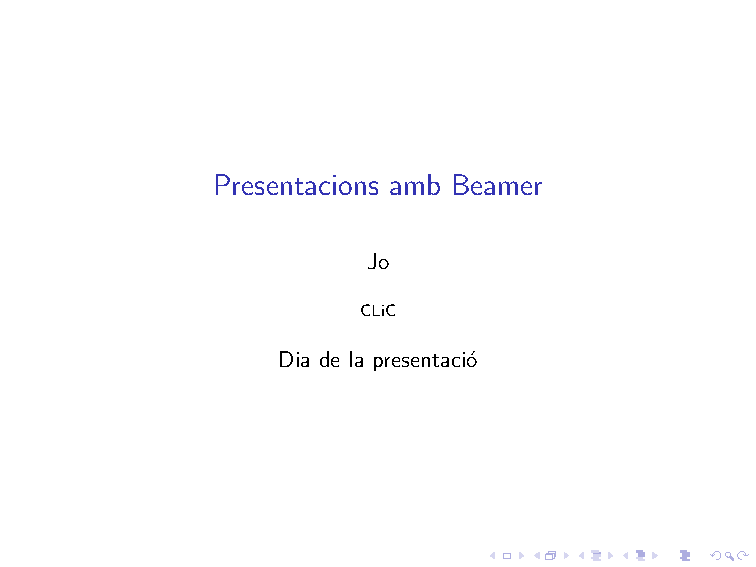
\includegraphics[width=\textwidth,clip,trim=1in 1in 1in 1in]{beamer-minimal.pdf}
\end{minipage}
\end{frame}

%%%%%%%%%%%%%%%%%%%%%%%%%%%%%%%%%%%%%%%%%%%%%%%%%%%%%%%%%%%%%%%%%%%%%%%%%%%%%%%
%%%%%%%%%%%%%%%%%%%%%%%%%%%%%%%%%%%%%%%%%%%%%%%%%%%%%%%%%%%%%%%%%%%%%%%%%%%%%%%
%%%%%%%%%%%%%%%%%%%%%%%%%%%%%%%%%%%%%%%%%%%%%%%%%%%%%%%%%%%%%%%%%%%%%%%%%%%%%%%
\begin{frame}[fragile]{Presentacions amb \protect\bftt{beamer}}

\begin{itemize}
\item Podeu partir de l'exemple i anar provant coses.
\end{itemize}
\vskip 2ex
\begin{center}
\fbox{\href{\wlnewdoc{beamer-minimal.tex}}{%
Click to open the example document in \wllogo{}}}
\end{center}
\end{frame}

%%%%%%%%%%%%%%%%%%%%%%%%%%%%%%%%%%%%%%%%%%%%%%%%%%%%%%%%%%%%%%%%%%%%%%%%%%%%%%%
%%%%%%%%%%%%%%%%%%%%%%%%%%%%%%%%%%%%%%%%%%%%%%%%%%%%%%%%%%%%%%%%%%%%%%%%%%%%%%%
%%%%%%%%%%%%%%%%%%%%%%%%%%%%%%%%%%%%%%%%%%%%%%%%%%%%%%%%%%%%%%%%%%%%%%%%%%%%%%%
\subsection{Marcs}
\begin{frame}[fragile]
\frametitle{Presentation amb \protect\bftt{beamer}: Marcs}
\begin{itemize}
\item Use \cmdbs{frametitle} to give the frame a title.
\item Then add content to the frame.
\item The source for this frame looks like:
\vskip 2ex
\inputminted[fontsize=\scriptsize,frame=single,resetmargins]{latex}%
  {beamer-frame.tex}
\end{itemize}
\end{frame}

%%%%%%%%%%%%%%%%%%%%%%%%%%%%%%%%%%%%%%%%%%%%%%%%%%%%%%%%%%%%%%%%%%%%%%%%%%%%%%%
%%%%%%%%%%%%%%%%%%%%%%%%%%%%%%%%%%%%%%%%%%%%%%%%%%%%%%%%%%%%%%%%%%%%%%%%%%%%%%%
%%%%%%%%%%%%%%%%%%%%%%%%%%%%%%%%%%%%%%%%%%%%%%%%%%%%%%%%%%%%%%%%%%%%%%%%%%%%%%%
\subsection{Seccions}
\begin{frame}[fragile]{Presentation amb \protect\bftt{beamer}: Seccions}
\begin{itemize}
\item You can use \cmdbs{section}s to group your \bftt{frame}s, i
\bftt{beamer} will use them to create an automatic outline.
\item To generate an outline, use the \cmdbs{tableofcontents} ordre. Here's
one for this presentation. The \bftt{currentsection} option highlights the current section.
\vskip 2ex
\begin{exampletwouptiny}
% comentaris

% per

% guanyar 

% espai

\tableofcontents[currentsection]
\end{exampletwouptiny}
\end{itemize}
\end{frame}

%%%%%%%%%%%%%%%%%%%%%%%%%%%%%%%%%%%%%%%%%%%%%%%%%%%%%%%%%%%%%%%%%%%%%%%%%%%%%%%
%%%%%%%%%%%%%%%%%%%%%%%%%%%%%%%%%%%%%%%%%%%%%%%%%%%%%%%%%%%%%%%%%%%%%%%%%%%%%%%
%%%%%%%%%%%%%%%%%%%%%%%%%%%%%%%%%%%%%%%%%%%%%%%%%%%%%%%%%%%%%%%%%%%%%%%%%%%%%%%
\subsection{Columnes}
\begin{frame}[fragile]{Presentation amb \protect\bftt{beamer}: Multiple Columns}
\begin{columns}
\begin{column}{0.4\textwidth}
\begin{itemize}
\item Use the \bftt{columns} i \bftt{column} environments to break the slide
into columns.
\item The argument for each \bftt{column} determines its width.
\item See also the \bftt{multicol} package, which automatically breaks your
content into columns.
\end{itemize}
\end{column}
\begin{column}{0.6\textwidth}
\begin{minted}[fontsize=\scriptsize,frame=single]{latex}
\begin{columns}
  \begin{column}{0.4\textwidth}
    \begin{itemize}
    \item Use the columns ...
    \item The argument ...
    \item See also the ...
    \end{itemize}
  \end{column}
  \begin{column}{0.6\textwidth}
    % second column
  \end{column}
\end{columns}
\end{minted}
\end{column}
\end{columns}
\end{frame}

%%%%%%%%%%%%%%%%%%%%%%%%%%%%%%%%%%%%%%%%%%%%%%%%%%%%%%%%%%%%%%%%%%%%%%%%%%%%%%%
%%%%%%%%%%%%%%%%%%%%%%%%%%%%%%%%%%%%%%%%%%%%%%%%%%%%%%%%%%%%%%%%%%%%%%%%%%%%%%%
%%%%%%%%%%%%%%%%%%%%%%%%%%%%%%%%%%%%%%%%%%%%%%%%%%%%%%%%%%%%%%%%%%%%%%%%%%%%%%%
\begin{frame}[fragile]{Presentation amb \protect\bftt{beamer}: Destacar}
\begin{itemize}

\item Use \cmdbs{emph} or \cmdbs{alert} to highlight:
\vskip 1ex
\begin{exampletwouptiny}
I should \emph{emphasise} that
this is an \alert{important} point.
\end{exampletwouptiny}
\vskip 1ex

\item Or specify bold face or italics:
\vskip 1ex
\begin{exampletwouptiny}
Text in \textbf{bold face}.
Text in \textit{italics}.
\end{exampletwouptiny}
\vskip 1ex

\item Or specify a color (American spelling):
\vskip 1ex
\begin{exampletwouptiny}
It \textcolor{red}{stops}
and \textcolor{green}{starts}.
\end{exampletwouptiny}
\vskip 1ex
\item See \url{http://www.math.umbc.edu/~rouben/beamer/quickstart-Z-H-25.html}
for more colors \& custom colors.
\end{itemize}
\end{frame}

%%%%%%%%%%%%%%%%%%%%%%%%%%%%%%%%%%%%%%%%%%%%%%%%%%%%%%%%%%%%%%%%%%%%%%%%%%%%%%%
%%%%%%%%%%%%%%%%%%%%%%%%%%%%%%%%%%%%%%%%%%%%%%%%%%%%%%%%%%%%%%%%%%%%%%%%%%%%%%%
%%%%%%%%%%%%%%%%%%%%%%%%%%%%%%%%%%%%%%%%%%%%%%%%%%%%%%%%%%%%%%%%%%%%%%%%%%%%%%%
\subsection{Figures}
\begin{frame}[fragile]{Presentation amb \protect\bftt{beamer}: Figures}
\begin{itemize}
\item Use \cmdbs{includegraphics} from the \bftt{graphicx} package.
\item The \bftt{figure} environment centers by default, in \bftt{beamer}.
\vskip 2ex
\begin{exampletwouptiny}
\begin{figure}

\includegraphics[
  width=0.5\textwidth]{gus_gran}
\end{figure}
\end{exampletwouptiny}
\end{itemize}

\end{frame}

%%%%%%%%%%%%%%%%%%%%%%%%%%%%%%%%%%%%%%%%%%%%%%%%%%%%%%%%%%%%%%%%%%%%%%%%%%%%%%%
%%%%%%%%%%%%%%%%%%%%%%%%%%%%%%%%%%%%%%%%%%%%%%%%%%%%%%%%%%%%%%%%%%%%%%%%%%%%%%%
%%%%%%%%%%%%%%%%%%%%%%%%%%%%%%%%%%%%%%%%%%%%%%%%%%%%%%%%%%%%%%%%%%%%%%%%%%%%%%%
\begin{frame}[fragile]{Presentation amb \protect\bftt{beamer}: Blocks}
\begin{itemize}
\item A \bftt{block} environment makes a titled box.
\begin{exampletwouptiny}
\begin{block}{Interesting Fact}
This is important.
\end{block}

\begin{alertblock}{Cautionary Tale}
This is really important!
\end{alertblock}
\end{exampletwouptiny}

\item How exactly they look depends on the theme\dots
\end{itemize}
\end{frame}

%%%%%%%%%%%%%%%%%%%%%%%%%%%%%%%%%%%%%%%%%%%%%%%%%%%%%%%%%%%%%%%%%%%%%%%%%%%%%%%
%%%%%%%%%%%%%%%%%%%%%%%%%%%%%%%%%%%%%%%%%%%%%%%%%%%%%%%%%%%%%%%%%%%%%%%%%%%%%%%
%%%%%%%%%%%%%%%%%%%%%%%%%%%%%%%%%%%%%%%%%%%%%%%%%%%%%%%%%%%%%%%%%%%%%%%%%%%%%%%
\begin{frame}[fragile]
    \frametitle{Presentation amb \protect\bftt{beamer}: Themes}
\begin{itemize}
\item Customise the look of your presentation using themes.
\item See \url{http://deic.uab.es/~iblanes/beamer_gallery/index_by_theme.html}
for a large collection of themes.
\end{itemize}
\begin{minipage}{0.55\linewidth}
\inputminted[fontsize=\scriptsize,frame=single,resetmargins]{latex}%
  {beamer-theme.tex}
\end{minipage}
\begin{minipage}{0.35\linewidth}
% trim: l b r t
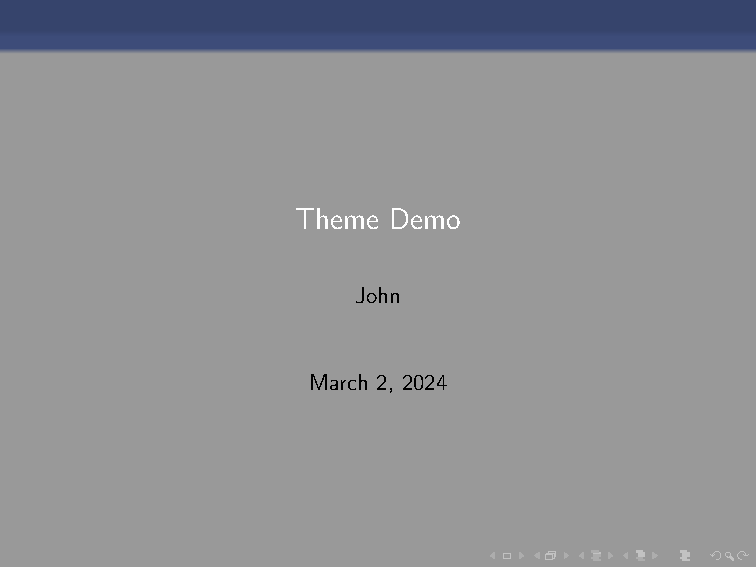
\includegraphics[width=\textwidth]{beamer-theme.pdf}
\end{minipage}
\end{frame}

%%%%%%%%%%%%%%%%%%%%%%%%%%%%%%%%%%%%%%%%%%%%%%%%%%%%%%%%%%%%%%%%%%%%%%%%%%%%%%%
%%%%%%%%%%%%%%%%%%%%%%%%%%%%%%%%%%%%%%%%%%%%%%%%%%%%%%%%%%%%%%%%%%%%%%%%%%%%%%%
%%%%%%%%%%%%%%%%%%%%%%%%%%%%%%%%%%%%%%%%%%%%%%%%%%%%%%%%%%%%%%%%%%%%%%%%%%%%%%%
\begin{frame}[fragile]{Presentation amb \protect\bftt{beamer}: Animation}
\begin{itemize}
\item A frame can generate multiple slides.
\item Use the \cmdbs{pause} ordre to show only part of a slide.
\vskip 2ex
\begin{exampletwouptinynoframe}
\begin{itemize}
\item Can you feel the 
\pause \item anticipation?
\end{itemize}
\end{exampletwouptinynoframe}
\vskip 2ex
\item There many more clever ways of making animations in \bftt{beamer}; see
also the \cmdbs{only}, \cmdbs{alt}, i \cmdbs{uncover} ordres.
\end{itemize}
\end{frame}

%%%%%%%%%%%%%%%%%%%%%%%%%%%%%%%%%%%%%%%%%%%%%%%%%%%%%%%%%%%%%%%%%%%%%%%%%%%%%%%
%%%%%%%%%%%%%%%%%%%%%%%%%%%%%%%%%%%%%%%%%%%%%%%%%%%%%%%%%%%%%%%%%%%%%%%%%%%%%%%
%%%%%%%%%%%%%%%%%%%%%%%%%%%%%%%%%%%%%%%%%%%%%%%%%%%%%%%%%%%%%%%%%%%%%%%%%%%%%%%
\begin{frame}[fragile]{Presentation amb \protect\bftt{beamer}: Exercise}

Recreate Peter Norvig's excellent ``Gettysburg Powerpoint Presentation'' in \bftt{beamer}.\footnote{\url{http://norvig.com/Gettysburg}}

\begin{enumerate}
\item Open this exercise in \wllogo{}:
\begin{center}
\fbox{\href{\wlnewdoc{beamer-exercise.tex}}{%
Click to open this exercise in \wllogo{}}}
\end{center}
\vskip 2ex
\item Download this image to your computer i upload it to \wllogo{} via the
files menu.
\begin{center}
\fbox{\href{\fileuri/gettysburg_graph.png?dl=1}{Click to download image}}
\end{center}
\vskip 2ex
\item Add \LaTeX{} ordres to the text to make it look like this one:
\begin{center}
\fbox{\href{\fileuri/beamer-exercise-solution.pdf}{%
Click to open the model document}}
\end{center}
\end{enumerate}
\end{frame}

%%%%%%%%%%%%%%%%%%%%%%%%%%%%%%%%%%%%%%%%%%%%%%%%%%%%%%%%%%%%%%%%%%%%%%%%%%%%%%%
%%%%%%%%%%%%%%%%%%%%%%%%%%%%%%%%%%%%%%%%%%%%%%%%%%%%%%%%%%%%%%%%%%%%%%%%%%%%%%%
%%%%%%%%%%%%%%%%%%%%%%%%%%%%%%%%%%%%%%%%%%%%%%%%%%%%%%%%%%%%%%%%%%%%%%%%%%%%%%%
\section{Què més?}
\begin{frame}{Continguts}
\begin{multicols}{2}
\tableofcontents[currentsection]
\end{multicols}
\end{frame}

%%%%%%%%%%%%%%%%%%%%%%%%%%%%%%%%%%%%%%%%%%%%%%%%%%%%%%%%%%%%%%%%%%%%%%%%%%%%%%%
%%%%%%%%%%%%%%%%%%%%%%%%%%%%%%%%%%%%%%%%%%%%%%%%%%%%%%%%%%%%%%%%%%%%%%%%%%%%%%%
%%%%%%%%%%%%%%%%%%%%%%%%%%%%%%%%%%%%%%%%%%%%%%%%%%%%%%%%%%%%%%%%%%%%%%%%%%%%%%%
\subsection{Altres coses interessants}
\begin{frame}[fragile]{Altres}
\begin{itemize}
\item L'ordre \cmdbs{tableofcontents} genera un índex automàticament a partir
dels títols de les seccions i subseccions.

\item Change the \cmdbs{documentclass} to
\mint{latex}!\documentclass{scrartcl}!
or
\mint{latex}!\documentclass[12pt]{IEEEtran}!

\item Define your own ordre for a complicated equation:
\begin{exampletwouptiny}
\newcommand{\rperf}{%
  \rho_{\text{perf}}}
$$
\rperf = {\bf c}'{\bf X} + \varepsilon
$$
\end{exampletwouptiny}
\end{itemize}
\end{frame}

%%%%%%%%%%%%%%%%%%%%%%%%%%%%%%%%%%%%%%%%%%%%%%%%%%%%%%%%%%%%%%%%%%%%%%%%%%%%%%%
%%%%%%%%%%%%%%%%%%%%%%%%%%%%%%%%%%%%%%%%%%%%%%%%%%%%%%%%%%%%%%%%%%%%%%%%%%%%%%%
%%%%%%%%%%%%%%%%%%%%%%%%%%%%%%%%%%%%%%%%%%%%%%%%%%%%%%%%%%%%%%%%%%%%%%%%%%%%%%%
\subsection{Altres paquets}
\begin{frame}{Altres paquets}
\begin{itemize}
\item \bftt{tikz}: gràfics, una mica difícil.
\item \bftt{tikz-qtree}: arbres per sintaxi, relacions genètiques \dots
\item \bftt{pgfplots}: create graphs in \LaTeX
\item \bftt{langnames}: per noms d'idiomes de manera sistemàtica.
\end{itemize}
Vegeu \url{https://www.overleaf.com/latex/examples} i \url{http://texample.net}
per exemples.
\end{frame}

%%%%%%%%%%%%%%%%%%%%%%%%%%%%%%%%%%%%%%%%%%%%%%%%%%%%%%%%%%%%%%%%%%%%%%%%%%%%%%%
%%%%%%%%%%%%%%%%%%%%%%%%%%%%%%%%%%%%%%%%%%%%%%%%%%%%%%%%%%%%%%%%%%%%%%%%%%%%%%%
%%%%%%%%%%%%%%%%%%%%%%%%%%%%%%%%%%%%%%%%%%%%%%%%%%%%%%%%%%%%%%%%%%%%%%%%%%%%%%%
\subsection{Instalar \LaTeX{}}
\begin{frame}{Instalar \LaTeX}
\begin{itemize}
\item Per fer servir \LaTeX{} al vostre ordinador, us caldrà una \emph{distribució}:
    inclou el programa \bftt{latex} i un munt de paquets.
\begin{itemize}
\item Windows: \href{http://miktex.org/}{Mik\TeX} o \href{http://tug.org/texlive/}{\TeX Live}
\item Linux: \href{http://tug.org/texlive/}{\TeX Live}
\item Mac: \href{http://tug.org/mactex/}{Mac\TeX}
\end{itemize}
\item També us caldrà un editor amb suport per \LaTeX{}. A \url{http://en.wikipedia.org/wiki/Comparison_of_TeX_editors} hi teniu una llista exhaustiva.
\end{itemize}
\end{frame}

%%%%%%%%%%%%%%%%%%%%%%%%%%%%%%%%%%%%%%%%%%%%%%%%%%%%%%%%%%%%%%%%%%%%%%%%%%%%%%%
%%%%%%%%%%%%%%%%%%%%%%%%%%%%%%%%%%%%%%%%%%%%%%%%%%%%%%%%%%%%%%%%%%%%%%%%%%%%%%%
%%%%%%%%%%%%%%%%%%%%%%%%%%%%%%%%%%%%%%%%%%%%%%%%%%%%%%%%%%%%%%%%%%%%%%%%%%%%%%%
\subsection{Exemples comentats}
\begin{frame}{Exemples comentats}
De senzill a complex:
\begin{itemize}
    \item \href{https://www.overleaf.com/read/rgxbsfvqsgbw\#ba04b9}{Breu transcripció fonètica} --- amb \bftt{tipauni} o \bftt{tipa} (comentat).
    \item \href{https://www.overleaf.com/read/mxysfjcnnppm\#294a25}{Treball de transcripció fonètica} --- més extens que l'anterior, barreja de \bftt{tipa} i unicode.
    \item \href{https://www.overleaf.com/read/sxkcdfrpmbcb\#10abd3}{Treball morfologia basca} --- conté:
\begin{itemize}
    \item Un treball estructurat amb diversos fitxers, glosses personalitzades, taules amb format avançat i exemples de bibliografia tant amb biblatex com amb apacite.
    \item Una presentació amb \bftt{beamer}.
\end{itemize}
\end{itemize}

Finalment, us pot ser útil \href{https://www.overleaf.com/read/vsdvmbzywdrn\#d43fce}{aquesta plantilla senzilla}.

\end{frame}

%%%%%%%%%%%%%%%%%%%%%%%%%%%%%%%%%%%%%%%%%%%%%%%%%%%%%%%%%%%%%%%%%%%%%%%%%%%%%%%
%%%%%%%%%%%%%%%%%%%%%%%%%%%%%%%%%%%%%%%%%%%%%%%%%%%%%%%%%%%%%%%%%%%%%%%%%%%%%%%
%%%%%%%%%%%%%%%%%%%%%%%%%%%%%%%%%%%%%%%%%%%%%%%%%%%%%%%%%%%%%%%%%%%%%%%%%%%%%%%
\subsection{Referències en línia}
\begin{frame}{Referències en línia}
\begin{itemize}
\item \href{https://www.overleaf.com/learn}{The Overleaf Learn Wiki} --- tutorials i material de referència.
\item \href{http://en.wikibooks.org/wiki/LaTeX}{The \LaTeX{} Wikibook} --- més tutorials i material de referència.
\item \href{http://tex.stackexchange.com/}{\TeX{} Stack Exchange} --- preguntes i respostes
\item \href{http://www.latex-community.org/}{\LaTeX{} Community} --- fòrum
\item \href{http://ctan.org/}{Comprehensive \TeX{} Archive Network (CTAN)} --- documentació de paquets.
\item Qualsevol buscador us portarà a alguna d'aquestes pàgines.
\end{itemize}

Repositori del curs: \href{https://github.com/Pastells/curs-latex}{Pastells/curs-latex}
\end{frame}


%%%%%%%%%%%%%%%%%%%%%%%%%%%%%%%%%%%%%%%%%%%%%%%%%%%%%%%%%%%%%%%%%%%%%%%%%%%%%%%
%%%%%%%%%%%%%%%%%%%%%%%%%%%%%%%%%%%%%%%%%%%%%%%%%%%%%%%%%%%%%%%%%%%%%%%%%%%%%%%
%%%%%%%%%%%%%%%%%%%%%%%%%%%%%%%%%%%%%%%%%%%%%%%%%%%%%%%%%%%%%%%%%%%%%%%%%%%%%%%
\begin{frame}[standout]
\Huge Gràcies!
\end{frame}

\end{document}
